\documentclass[twoside]{article}
\usepackage{graphicx}
\usepackage{polski}
\usepackage{fancyhdr}
\usepackage{lastpage}
\usepackage{epigraph}
\usepackage{listings}
\usepackage{soul}
\usepackage{color}
\usepackage{multirow}
\usepackage{subcaption}
\usepackage{fancyvrb}
\usepackage{hyperref}


\title{AiSD Ex. 3 (Wt.)}
\author{\hl{Mateusz Kamieniecki}}
\date{\today}

\lstset{
    numbers=left
}

\makeatletter

\begin{document}

\pagestyle{fancy}
\fancyhead{}
\fancyhead[L]{\@title}
\fancyhead[R]{\@author}
\fancyhead[C]{\@date}

\cfoot{\thepage\ / \pageref{LastPage}}


\newpage

\section{Wprowadzenie}

\epigraph{
Wybudować grób.
To się tylko tak mówi.
A kto nie budował, ten nie wie, co taki grób kosztuje.
Prawie tyle co dom.
Choć grób, mówią, też dom, tylko że na tamto życie.
Bo wieczność nie wieczność, a~swój kąt powinien człowiek mieć
}{Wiesław Myśliwski, \textit{Kamień na kamieniu}}

,,(...) Bo wieczność nie wieczność, a swój kąt powinien człowiek mieć. (...)'' napisał Wiesław Myśliwski w Kamieniu na kamieniu.
I choć to zdanie pojawia się tutaj tylko dlatego, że czasami trzeba efektownie zacząć,
to... może to wcale nie jest przypadek?

Tablice mieszające z rozwiązywaniem kolizji metodą łańcuchową w teorii powinny zapewnić nam
wykonywanie operacji (dodawania, wyciągania i usuwania elementów) ze stałą złożonością $O(1)$
niezależną od liczby przechowywanych elementów.
Tyle teoria.
W praktyce sprawdziliśmy, że tablice są efektywne, a przy odpowiedniej implementacji funkcji
haszujących udaje się spełnić warunek oczekiwanej złożoności czasowej, na którą oczywiście
wpływa aktualna wartość współczynnika zapełnienia tablicy $\alpha$, czyli stosunek liczby 
wszystkich wstawionych elementów do rozmiaru tablicy mieszającej.
Wadą rozważanej przez nas implementacji było występowanie kolizji początkowo zgodne 
z prawdopodobieństwem jego wystąpienia (gdy $\alpha < 1$), a w późniejszej fazie wymuszone
przez brak wolnych indeksów (czyli pustych łańcuchów) w naszej tablicy (gdy $\alpha > 1$).

A co mogłoby się stać, gdyby każdy element -- niczym człowiek u W. Myśliwskiego -- ,,swój kąt 
powinien mieć''?
Postawmy to pytanie nieco bardziej przyziemnie: czy przy rozwiązywaniu kolizji trzeba korzystać
z metody łańcuchowej?
Nie czekając zbyt długo możemy odpowiedzieć: nie, nie trzeba.
Innym pomysłem na poradzenie sobie z sytuacją, gdy dochodzi do kolizji (gdy dla dwóch kluczy 
(elementów) otrzymujemy taką samą wartość haszującą) jest \textbf{adresowanie otwarte}.

W tym podejściu wszystkie elementy są wprost przechowywane w tablicy, czyli nie tworzymy żadnych
list do przeszukiwania i łączenia kluczy (elementów) o takiej samej wartości haszującej.
W takim razie, jeśli elementy są umieszczane bezpośrednio w tablicy pod wyliczonymi indeksami, to
należy sprawdzić, co się stanie, gdy wystąpi kolizji (która niewątpliwie nie została cudownie
wyelimionwana przez samą zmianę nazwy metody).

Adresowanie otwarte, zamiast rozważania pojedynczego indeksu wyliczonego na podstawie klucza,
oblicza ciąg pozycji (na podstawie klucza), które są potencjalnymi indeksami (miejscami) docelowymi
dla analizowanego elementu (klucza).
A z tego ciągu potencjalnych indeksów, w przypadku wstawiania nowego elementu do tablicy 
mieszającej, wybierany jest pierwszy wolny (niezapisany) indeks.
Przy wyszukiwaniu proces wygląda podobnie: przeszukujemy ciąg indeksów (wyznaczonych na podstawie 
klucza), pod którymi potencjalnie może być umieszczony poszukiwany element.
Jeżeli po drodze trafimy na puste miejsce w tablicy lub przejrzymy wszystkie indeksy (w wyznaczonej 
kolejności), to stwierdzamy, że poszukiwany element nie występuje w tablicy.
Zostało to pokazane na rysunku \ref{fig:linear-probing-label}.

\begin{figure}[ht!]
    \centerline{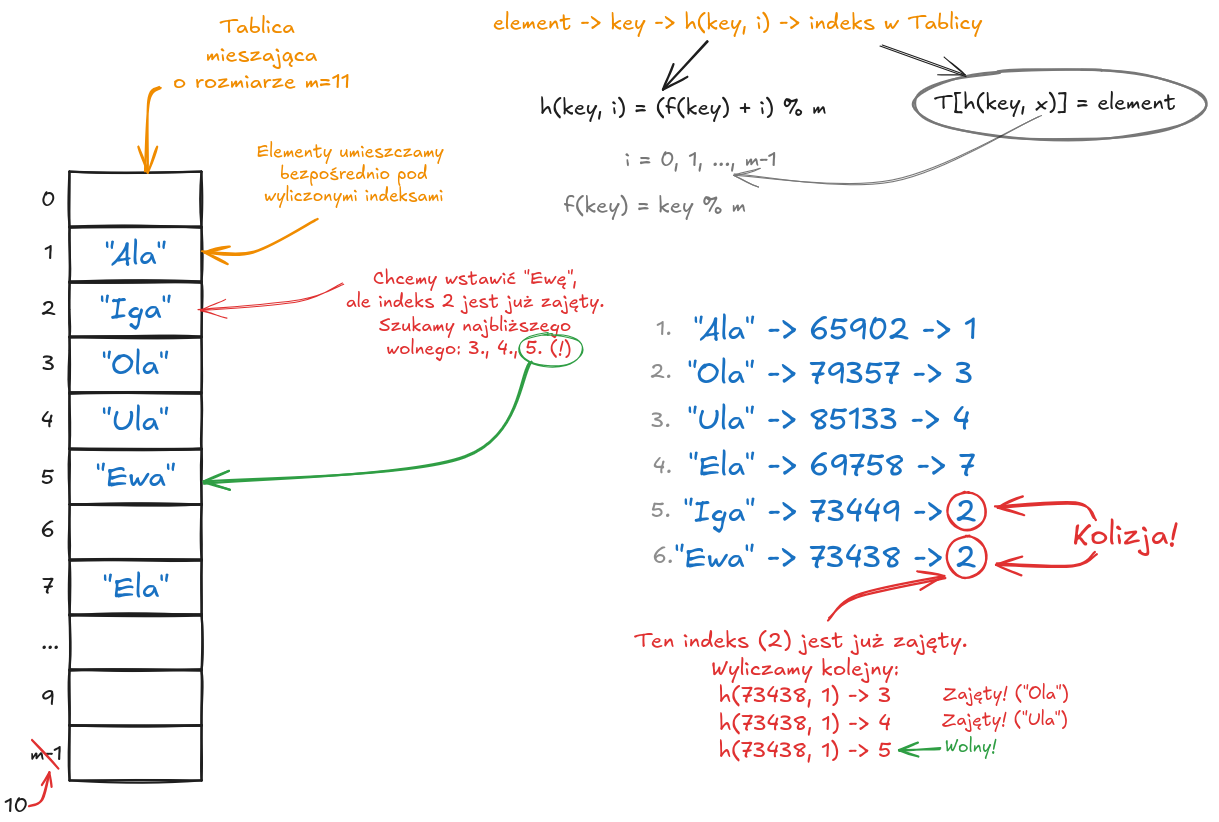
\includegraphics[width=1.5\linewidth]{images/1_linear_probing.png}}
    \caption{Przedstawienie procesu wstawiania kolejnych elementów do tablicy mieszającej.
    Pierwsze wartości (Ala, Ola, Ula, Ela, Iga) trafiają bezpośrednio pod wyliczone indeksy.
    W przypadku ostatniej wstawianej wartości dochodzi do kolizji (indeks 2. wyliczony dla ,,Ewy''
    jest już zajęty), dlatego potrzebne jest przejęcie przez kolejne wartości ciągu kontrolnego.
    Ostatecznie ,,Ewa'' zostaje umieszczona pod indeksem 5. (po sprawdzeniu: 2., 3., 4.,).
    Do wyliczenia indeksów została użyta funkcja adresowania liniowego przy rozmiarze tablicy $m=11$.}
    \label{fig:linear-probing-label}
\end{figure}

Sprawa nieco bardziej komplikuje się, gdy usuwamy element z tablicy mieszającej.
Wtedy nie wystarczy odnaleźć indeksu, pod którym znajduje się poszukiwany element, a następnie
zamienić go na wartość \verb|NIL| (oznaczającą wartość pustą).
Dlaczego?
Ponieważ usunięty element może zaburzyć porządek poszukiwania innych elementów, które miały z nim
kolizję (i zostały umieszczone na dalszych pozycjach ze swoich wyliczonych ciągów).
Dla lepszego zrozumienia tej sytuacji, spójrzmy na rysunek \ref{fig:deleting-and-searching-label}.

\begin{figure}[ht!]
    \centerline{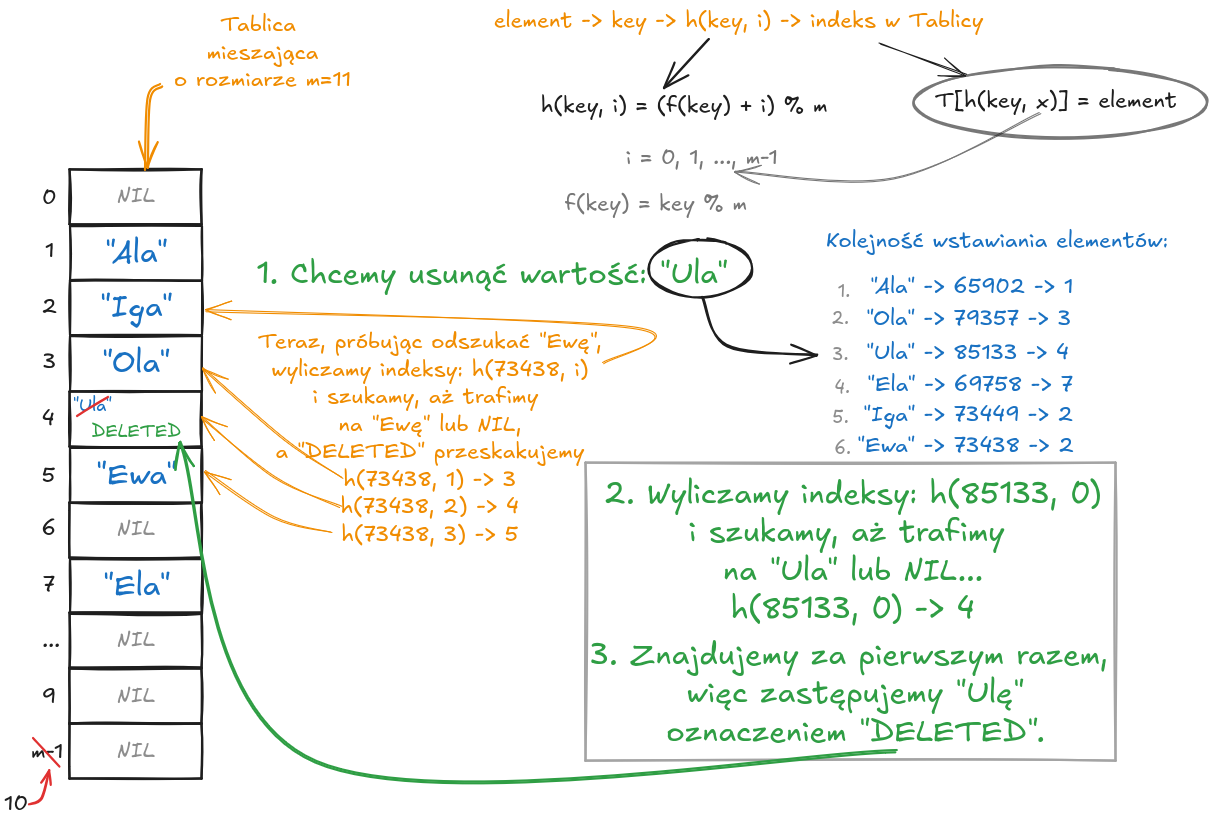
\includegraphics[width=1.5\linewidth]{images/2_linear_probing_deleting_and_searching.png}}
    \caption{Przedstawiono dwie operacje: usunięcia wartości ,,Ula'', odszukania wartości ,,Ewa''.
    ,,Ulę'' odnajdujemy od razu i usuwamy ją poprzez wpisanie do tablicy pod indeksem $i=4$ 
    wartości ,,DELETED''. Dzięki temu podczas wyszukiwania wartości ta komórka zostanie potraktowana jako zajęta, a podczas wstawiania nowego elementu -- jako pusta.
    Szukając ,,Ewy'' przeskakujemy komórkę pod indeksem $i=4$ i odnajdujemy ,,Ewę'' pod indeksem 
    $i=5$.}
    \label{fig:deleting-and-searching-label}
\end{figure}

W związku z tym usuwany element należy zastąpić innym, specjalnym elementem, który będzie oznaczał,
że w przypadku operacji wyszukiwania (innego elementu) nie należy przerywać procesu
(uznajemy, że ten indeks nie jest pusty, a po prostu nie odpowiada wyszukiwanemu elementowi),
a w przypadku operacji wstawiania ten element będzie traktowany jako oznaczenie pustego (wolnego)
miejsca w tablicy mieszającej.

\subsection{Obliczanie ciągów kontrolnych}
W adresowaniu otwartym zwykle stosuje się jeden z trzech popularnych sposobów wyliczania ciągów
kontrolnych, a zalicza się do nich: adresowanie liniowe, adresowanie kwadratowe, dwukrotne haszowanie.

Przy założeniu, że rozmiar tablicy mieszającej jest równy $m$, wyliczane ciągi kontrolne będą
permutacjami wszystkich indeksów tablicy mieszającej: $\{0, 1,$ $ ..., m-1\}$.

\subsubsection{Adresowanie liniowe}
Wykorzystując funkcję $f_1$ haszowania modularnego (charakterystyczną dla meteody łańcuchowej),
można przyjąć, że ciąg indeksów w adresowaniu liniowym jest wyliczany jako:

$$h(k, i) = (f_1(k) + i) \% m$$
$$f_1(k) = k \% m$$
, dla $i = 0, 1, ..., m-1$.

Niewątpliwą zaletą tej metody jest łatwość implementacji.
Wadę zaś stanowi występowanie zjawiska \textbf{grupowania pierwotnego}, 
które wynika z faktu, że im większa jest wartość współczynnika zapełnienia (im więcej elementów 
w tablicy), tym dłuższe ciągi zajętych indeksów występują w tablicy mieszającej, a tym samym 
element wstawiany jest na pierwszą wolną pozycję po przeszukaniu wielu wcześniejszych, 
zajętych indeksów.
To wprost przyczynia się do wydłużania średniego czasu trwania każdej operacji (wstawiania, 
wyszukiwania, usuwania).

\subsubsection{Adresowanie kwadratowe}
Z problemem grupowania lepiej radzi sobie adresowanie kwadratowe, w którym skok pomiędzy kolejnymi
indeksami (wartościami wyliczonego ciągu kontrolnego dla danego klucza $k$) jest zależny od
kwadratu numeru indeksu rozpatrywanej wartości ciągu kontrolnego:

$$h(k, i) = (f_1(k) + a \cdot i + b \cdot i^2) \% m$$
$$f_1(k) = k \% m$$
, dla $i = 0, 1, ..., m-1$.
Gdzie dodatkowy problem stanowi dobór stałych: $a$, $b$.

Chociaż kolejne wartości są od siebie bardziej oddalone niż w przypadku adresowania liniowego,
to w tym podejściu liczba różnych możliwych ciągów kontrolnych również jest równa $m$ (jest 
,,tylko'' $m$ indeksów, od których możemy rozpocząć wyliczenie ciągów kontrolnych).
Dodatkowo jeśli dla dwóch różnych kluczy wystąpi kolizja ($h(k_1, 0) == h(k_2, 0)$), 
to pozostałe wartości ciągu kontrolnego, również będą ze sobą kolidowały ($h(k_1, i) == h(k_2, i)$),
co w efekcie doprowadzi do (niepożądanego) \textbf{grupowania wtórnego}.

\subsubsection{Dwukrotne haszowanie}
Teoretycznie remedium na problemy (,,małą'' liczbę ciągów kontrolnych, grupowanie elementów)
jest funkcja dwukrotnego haszowania, w której -- jak nazwa wskazuje -- wykonuje się wyliczanie
hasza dwa razy (przy pomocy dwóch różnych funkcji):

$$h(k, i) = (f_1(k) + i \cdot f_2(k)) \% m$$
$$f_1(k) = k \% m$$
$$f_2(k) = 1 + (k \% (m - 1))$$
, dla $i = 0, 1, ..., m-1$.

Podane funkcje: $f_1$, $f_2$ stanowią oczywiście jedynie przykład.
Istotne jest jednak zwrócenie uwagi na kilka szczegółów.
Aby upewnić się, że otrzymany ciąg kontrolny będzie permutacją wszystkich indeksów tablicy 
mieszającej, należy zadbać o to, aby wartość $f_2$ była względnie pierwszą z $m$ 
($NWD(f_2(k), m) = 1$),
a można to osiągnąć czyniąc jak w powyższym przykładzie (przyjąć $m$ jako liczbę pierwszą, a
wartość $f_2$ ograniczyć do wartości mniejszych od $m$ ($m - 1$).
Przy spełnieniu tych warunków funkcja dwukrotnego haszowania powinna dostarczać $\Theta(m^2)$
ciągów kontrolnych -- każda para $(f_1(k), f_2(k))$ daje inny ciąg kontrolny.



\section{Zadania}

\subsection{Zadanie 0}
Proszę uporządkować swoje repozytorium, aby organizacja projektów wyglądała jak poniżej. 
Oczywiście w tej strukturze mogą znajdować się również inne katalogi i pliki, ale proszę
dokładnie odwzorować przedstawiony porządek projektów.

\begin{verbatim}
.korzeń_repozytorium
+-- CW_0
|   |
|   +-- pliki_i_katalogi_z_zajęć
|
+-- CW_1
|   +-- AiSD2026ZEx1
|       +-- pom.xml
|
+-- CW_2
|   +-- AiSD2026ZEx2
|       +-- pom.xml
|
+-- CW_3
    +-- AiSD2026ZEx3
        +-- pom.xml
\end{verbatim}

\newpage

%---------------------------------------------------------
% Please, use this tool: https://www.tablesgenerator.com/#
%---------------------------------------------------------
\subsection{Zadanie 1}

Proszę porównać czas działania i liczbę wykonanych operacji (\verb|put(...)|, \verb|hashFunc(...)|,
\verb|doubleResize(...)|) w zależności od: metody haszowania, źródła danych.
Rozważyć należy:
\begin{itemize}
    \item metody: haszowania liniowego, dwukrotnego haszowania;
    \item dane: losowe łańcuchy znaków, dane z pliku 
(\href{https://www.mit.edu/~ecprice/wordlist.100000}{źródło MIT}).
\end{itemize}

\begin{table}[h]
\begin{tabular}{|l|l|l|l||l|l|l|}
\hline
Lp. & Rozmiar & Czas[ms] & Końcowy wsp. $\alpha$ & put(...) & hashFunc(...) & doubleResize(...) \\ \hline
1. & 5101 & & & & & \\ \hline
2. & 8297 &  &  &  &  &  \\ \hline
3. & 16493 &  &  &  &  &  \\ \hline
4. & 32909 &  &  &  &  &  \\ \hline
5. & 65651 &  &  &  &  &  \\ \hline
6. & 131111 &  &  &  &  &  \\ \hline
7. & 263023 &  &  &  &  &  \\ \hline
8. & 524309 &  &  &  &  &  \\ \hline
\end{tabular}
\caption{Czas (i liczba) wykonywania operacji podczas wkładania \textbf{losowych danych} do
tablicy mieszającej z \textbf{adresowaniem liniowym}.}
\end{table}

\begin{table}[h]
\begin{tabular}{|l|l|l|l||l|l|l|}
\hline
Lp. & Rozmiar & Czas[ms] & Końcowy wsp. $\alpha$ & put(...) & hashFunc(...) & doubleResize(...) \\ \hline
1. & 5101 & 1352 & 0,61262 & 218599 & 14039563 & 5 \\ \hline
2. & 8297 & 884 & 0,37664  & 292906  & 23239711  & 5  \\ \hline
3. & 16493 &  &  &  &  &  \\ \hline
4. & 32909 &  &  &  &  &  \\ \hline
5. & 65651 &  &  &  &  &  \\ \hline
6. & 131111 &  &  &  &  &  \\ \hline
7. & 263023 &  &  &  &  &  \\ \hline
8. & 524309 &  &  &  &  &  \\ \hline
\end{tabular}
\caption{Czas (i liczba) wykonywania operacji podczas wkładania \textbf{danych z pliku} (MIT) do
tablicy mieszającej z \textbf{adresowaniem liniowym}.}
\end{table}

\begin{table}[h]
\begin{tabular}{|l|l|l|l||l|l|l|}
\hline
Lp. & Rozmiar & Czas & Końcowy wsp. $\alpha$ & put(...) & hashFunc(...) & doubleResize(...) \\ \hline
1. & 5101 &  &  &  &  &  \\ \hline
2. & 8297 &  &  &  &  &  \\ \hline
3. & 16493 &  &  &  &  &  \\ \hline
4. & 32909 &  &  &  &  &  \\ \hline
5. & 65651 &  &  &  &  &  \\ \hline
6. & 131111 &  &  &  &  &  \\ \hline
7. & 263023 &  &  &  &  &  \\ \hline
8. & 524309 &  &  &  &  &  \\ \hline
\end{tabular}
\caption{Czas (i liczba) wykonywania operacji podczas wkładania \textbf{danych z pliku} (MIT) do
tablicy mieszającej z \textbf{dwukrotnym haszowaniem}.}
\end{table}

\noindent \textbf{Komentarz do otrzymanych wyników (z trzech tabel):} \hl{TODO ------------------}.

\newpage

\subsection{Zadanie 2}
W pakiecie testowym \verb|pl.edu.pw.ee.aisd2025zex3.performance.clustering| są cztery konkretne klasy do uruchomienia (jest sześć, ale nas interesują cztery). Wynikiem ich uruchomienia jest plik \verb|PNG|, w którym czarne piksele są odzwierciedleniem wolnych komórek w tablicy mieszającej, a białe piksele -- komórek zajętych.

Plik jest zapisywany wierszami (czyli gdybyśmy pocięli ten plik na paski o szerokości jednego piksela i połączyli je, to otrzymalibyśmy ,,wizualizację'' tablicy mieszającej).

Proszę utworzyć cztery obrazki wynikowe (zapisują się w korzeniu projektu) i zinterpretować je (proszę uzupełnić miejsce na komentarz).

\begin{figure}
    \centering
    
    \begin{subfigure}[b]{0.49\textwidth}
        \centering
        \includegraphics[width=\textwidth]{example-image}
        \caption[]{{Adresowanie liniowe, dane MIT}}
    \end{subfigure}    
    \hfill    
    \begin{subfigure}[b]{0.49\textwidth}
        \centering
        \includegraphics[width=\textwidth]{example-image}
        \caption[]{{Adresowanie liniowe, dane ,,losowe''}}
    \end{subfigure}    
    \vskip\baselineskip    
    \begin{subfigure}[b]{0.49\textwidth}
        \centering
        \includegraphics[width=\textwidth]{example-image}
        \caption[]{{Haszowanie dwukrotne, dane MIT}}
    \end{subfigure}    
    \hfill    
    \begin{subfigure}[b]{0.49\textwidth}
        \centering
        \includegraphics[width=\textwidth]{example-image}
        \caption[]{{Haszowanie dwukrotne, dane ,,losowe''}}
    \end{subfigure}
    
    \caption{,,Wizualizacja'' wypełnienia hasza w zależności od typu danych i funkcji haszującej.\ (Białe piksele oznaczają zapełnione komórki, a czarne -- puste.)}
\end{figure}

\noindent \textbf{Komentarz do otrzymanych wizualizacji:} \hl{TODO ------------------}.

\newpage

\subsection{Zadanie 3}
Wykorzystując pakiet testowy \verb|pl.edu.pw.ee.aisd2026zex3.performance.clustering|
proszę przygotować wizualizacje zapełniania tablic mieszających dla adresowania kwadratowego.

Proszę ręcznie dobierać (i zapisać!) stałe $a$ oraz $b$ w celu znalezienia najkorzystniejszego 
wyniku. 
Potrzebna będzie cierpliwość, intuicja i odrobina szczęścia.

Proszę skupić się głównie na danych z MIT \\
(klasa: \verb|HashQuadraticProbingMitWordsClusteringVisualization|).
Dla znalezionej najlepszej pary stałych ($a$, $b$), proszę dodatkowo wykonać jedną wizualizację
dla danych  losowych\\
(klasa: \verb|HashQuadraticProbingRandWordsClusteringVisualization|).

Proszę uzupełnić miejsce na komentarz (wnioski).

\begin{figure}
    \centering

    \begin{subfigure}[b]{0.49\textwidth}
        \centering
        \includegraphics[width=\textwidth]{example-image}
        \caption[]{{Set\_1. Dane \textbf{MIT}. \hl{a=??? $|$ b=???}}}
    \end{subfigure}
    \hfill
    \begin{subfigure}[b]{0.49\textwidth}
        \centering
        \includegraphics[width=\textwidth]{example-image}
        \caption[]{{Set\_2. Dane \textbf{MIT}. \hl{a=??? $|$ b=???}}}
    \end{subfigure}
    \vskip\baselineskip
    \begin{subfigure}[b]{0.49\textwidth}
        \centering
        \includegraphics[width=\textwidth]{example-image}
        \caption[]{{Set\_3. Dane \textbf{MIT}. \hl{a=??? $|$ b=???}}}
    \end{subfigure}
    \hfill
    \begin{subfigure}[b]{0.49\textwidth}
        \centering
        \includegraphics[width=\textwidth]{example-image}
        \caption[]{{Set\_4. Dane \textbf{MIT}. \hl{a=??? $|$ b=???}}}
    \end{subfigure}
    \vskip\baselineskip
        \begin{subfigure}[b]{0.49\textwidth}
        \centering
        \includegraphics[width=\textwidth]{example-image}
        \caption[]{{Set\_\hl{???}. Dane \textbf{losowe}. \hl{a=??? $|$ b=???}}}
    \end{subfigure}

    \caption{,,Wizualizacja'' wypełnienia hasza przy \textbf{adresowaniu kwadratowym}.\
    Białe piksele oznaczają zapełnione komórki, a czarne -- puste.\
    Rysunki (a-d) pokazują wypełnienie dla danych MIT.\
    Rysunek (e) pokazuje wynik wypełnienia danymi losowymi, dla wartości $a$ oraz $b$\
    wybranych jako najlepsze z~pozostałych rysunków (a-d).}
    
\end{figure}

\noindent \textbf{Komentarz do otrzymanych wizualizacji:} \hl{TODO ------------------}.

\newpage

\subsection{Zadanie 4}
Proszę uzupełnić i przetestować implementację pod kątem wkładania, pobierania i usuwania
elementów z tablicy mieszającej.

\section{Na zakończenie}
To już prawie koniec, ale (dzisiaj, podobnie jak ostatnio) nie wolno nam zapomnieć, że:
\begin{itemize}
    \item wszystkie zmiany (cały kod źródłowy) muszą trafić do repozytorium;
    \item ostatnioą zmianę (\textit{commit}), przed końcem zajęć, należy oznaczyć tagiem ze znacznikiem czasowym \textbf{CW\_3\_EOT}.
    A~ostatnią zmianę (\textit{commit}) należy oznaczyć tagiem ze znacznikiem czasowym \textbf{CW\_3\_FINAL};
    \item końcową wersja tego dokumentu (PDF) należy umiecić w ISOD-zie.
\end{itemize}



\end{document}
